\documentclass{ctexart}

\author{李约瀚 \\ 14130140331 \\ qinka@live.com \\ qinka@qinka.pw}
\title{FPGA设计基础实验报告 (二)}

\usepackage{listings}
\usepackage[figuresright]{rotating}
\lstset{breaklines}

\begin{document}
    
        % Cover
        \thispagestyle{empty}
        \begin{center}
            \vspace*{4em}
            {\Huge\textbf{FPGA设计基础实验报告\\\vspace*{0.5em} (二)}}
            \vfill
            \begin{tabular}{c@{:}l}
                班级 & 1413014 \\
                学号 & 14130140331 \\ 
                姓名 & 李约瀚 \\ 
                教师 & 沈沛意 \\
            \end{tabular} 
            \vspace*{4em}\\
        \end{center}
        \newpage
        
       
        % Setting
        \setcounter{page}{0}
        \setcounter{section}{0}
        %\renewcommand\thesection{实验编号 1-\numeric{section} 题目: }
        %\renewcommand\thesubsection{}
        %\renewcommand\thesubsubsection{(\numeric{subsubsection})}

        %% Exp 2-1
        
        \section{数字时钟管理实验}
        
        \subsection{实验目的}
        \begin{itemize}
        \item 熟悉ISE软件,会使用ISE软件进行设计和仿真
        \item 学会Xilinx IP核生成工具的使用
        \item 学会数字时钟管理IP核的配置和使用
        \end{itemize}

        \subsection{实验步骤}

        \begin{itemize}
        \item 创建工程
        \item 设计输入
        \item 设计综合
        \item 设计仿真
        \end{itemize}

        \subsection{报告正文}

        \subsubsection{实验原理}

        IP核,也就是知识产权核(\verb|Intellectual Property|),
        是那些己验证的、可重利用的、具有某种确定功能的IC模块。
        分为软核(\verb|soft IP core|)、固核(\verb|firm IP core|)
        和硬核(\verb|hard IP core|)

        IP核将一些在数字电路中常用,但比较复杂的功能块,
        如FIR滤波器、SDRAM控制器、PCI接口等设计成可修改参数的模块,
        在设计可以直接调用,从而大大提高了设计的可重用性,
        在数字系统设计中得到了广泛的应用。

        目前,大型设计一般推荐使用同步时序电路。同步时序电路基于时钟触发沿设计,
        对时钟的周期、占空比、延时和抖动提出了更高的要求。
        为了满足同步时序设计的要求,一般在FPGA设计中采用全局时钟资源
        驱动设计的主时钟,以达到最低的时钟抖动和延迟。
       
        Xilinx在其FPGA系列芯片中都提供了高性能数字时钟管理器(DCM)模块,
        是管理和掌控时钟的专用模块,可以实现时钟的分频,倍频,去抖动,相移等操作。

        \paragraph{新建工程}

        打开 ISE 14.7之后,选择新建工程,将工程的路径设置好。
        在单击下一步之后,选择 Nexys3 的 Spartan6 XC6SLX16-CS324 芯片对应的配置。硬件描述语言选择 Verilog,其中的设计硬件用的描述语言是 Verilog。
        然后点击下一步之后进入工程信息页面并确认无误之后,点击完成结束工程的创建。

        \paragraph{设计输入}

        在菜单 \verb|Project| 中选择 \verb|New Source| 创建新的设计,并选择 \verb|Verilog Module| 创建文件。

        其中输入的设计文件是:
        \begin{lstlisting}[language=Verilog]
`timescale 1ns / 1ps
// Copyright (C) Xilinx
module top(
    input clk,
    input reset,
    output clk_out1,
    output clk_out2,
    output locked
    );
	 
dcm_core dcm0
   (// Clock in ports
    .CLK_IN1(clk),      // IN
    // Clock out ports
    .CLK_OUT1(clk_out1),     // OUT
    .CLK_OUT2(clk_out2),     // OUT
    // Status and control signals
    .RESET(reset),// IN
    .LOCKED(locked));      // OUT

endmodule
        \end{lstlisting}

        添加 IP 核,在菜单 \verb|Project| 中选择 \verb|New Source| 创建新的设计,并选择 \verb|IP (CORE Generator & Architecture Wizard)| 创建IP核。
        然后再\verb|FPGA Features and Design| 中找到 \verb|Clocking Wizard| 创建时钟。在配置页面中将输入频率设置为100MHz,然后在第二个页面中设置两个时钟。频率分别是50MHz 与 200MHz。第二个时钟的相位是180度。

        \paragraph{综合设计}

        在左侧的 \verb|Design| 面板中下方中 双击 \verb|Synthesize-XST| 开始综合过程。

        在左侧的 \verb|Design| 面板中的 \verb|Hierarchy| 中选中创建的 HDL 源文件,在下方的双击 \verb|View RTL Schematic| 查看电路。

        \paragraph{设计仿真}
        
        为工程文件添加仿真文件。在菜单 \verb|Project| 中选择 \verb|New Source| 创建新的设计,并选择 \verb|Verilog Test Fixture| 创键测试文件。

        在测试文件中添加 \lstinline|always #5 clk = ~clk;|
        \begin{lstlisting}
`timescale 1ns / 1ps

module test_bench;

	// Inputs
	reg clk;
	reg reset;

	// Outputs
	wire clk_out1;
	wire clk_out2;
	wire locked;

	// Instantiate the Unit Under Test (UUT)
	top uut (
		.clk(clk), 
		.reset(reset), 
		.clk_out1(clk_out1), 
		.clk_out2(clk_out2), 
		.locked(locked)
	);

	initial begin
		// Initialize Inputs
		clk = 0;
		reset = 0;

		// Wait 100 ns for global reset to finish
		#100;
 
		// Add stimulus here

	end
	
	always #5 clk = ~clk;
      
endmodule
        \end{lstlisting}

        然后在左边面板中选中\verb|Simulation|,在工程管理区选中测试代码,
        然后在过程管理区双击\verb|Simulate Behavioral Model|
        ,\verb|ISE|将启动\verb|ISE Simulator|,运行仿真。

        \subsubsection{结果}
        
        通过仿真软件,获得到了仿真的的波形,如图\ref{fig:report2-clock-1}所示。
        \begin{figure}
\centering
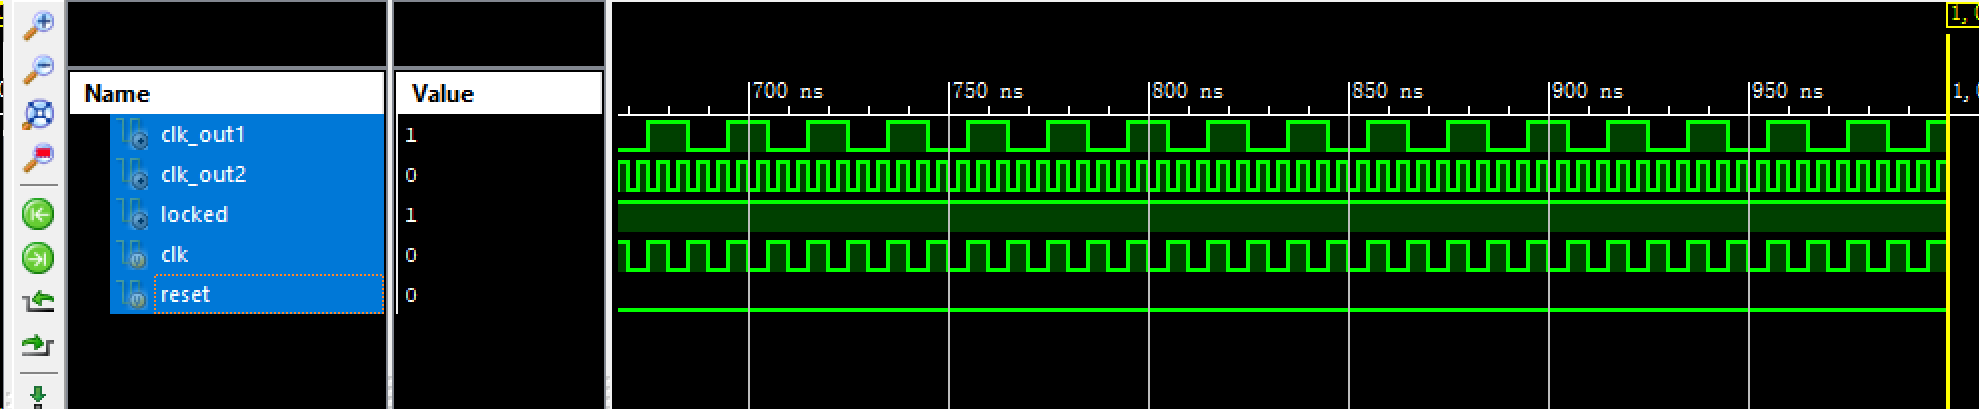
\includegraphics[width=1\linewidth]{report2-clock-1}
\caption{仿真波形}
\label{fig:report2-clock-1}
        \end{figure}


         %% Exp 2-2
         
         \section{VGA显示实验}
         
         \subsection{实验目的}
         \begin{itemize}
             \item 熟悉ISE软件,会使用ISE软件进行设计和仿真
             \item 了解VGA显示原理,熟悉DCM的应用
            \end{itemize}
            
            \subsection{实验步骤}
            
            \begin{itemize}
                \item 创建工程
                \item 设计输入
                \item 设计综合
                \item 进行硬件配置
                
            \end{itemize}
            
            \subsection{报告正文}
            
            \subsubsection{实验原理}
            
            Nexys3开发板上设置了VGA接口,通过15针接口连接到计算机的显示器。
            根据手册显示,VGA脚针与FPGA的对应关系如下:
            \begin{table}
                \centering
                \begin{tabular}{|c|c|c|}
                    \hline Pin 1  & Red[0:2]        & U7,V7,N7 \\ 
                    \hline Pin 2  & Green[0:2]      & P8,T6,V6 \\ 
                    \hline Pin 3  & Blue[1:2]       & R7,T7 \\ 
                    \hline Pin 4  &  &  \\ 
                    \hline Pin 5  & GND             &  \\ 
                    \hline Pin 6  & Red(GND)        &  \\ 
                    \hline Pin 7  & Green(GND)      &  \\ 
                    \hline Pin 8  & Blue(GND)       &  \\ 
                    \hline Pin 9  &  &  \\ 
                    \hline Pin 10 & Sync(GND)       &  \\ 
                    \hline Pin 11 &  &  \\ 
                    \hline Pin 12 &  &  \\ 
                    \hline Pin 13 & Horizontal Sync & N6 \\ 
                    \hline Pin 14 & Vertical Sync   & P7 \\ 
                    \hline Pin 15 &  &  \\ 
                    \hline 
                \end{tabular} 
                \caption{脚针对应关系}
            \end{table}
            
            对于阴极射线管的显示器,控制电子束打到荧光屏上形成一个像素点,电子束从左到右(称为水平扫描)和从上到下(称为垂直扫描),不断重复上述过程,在显示器上形成一幅图像。
            由于扫描的速度比较快,人眼看到的是一整幅图像,其实在某一时刻,只有一个像素点在发光。
            \begin{figure}
\centering
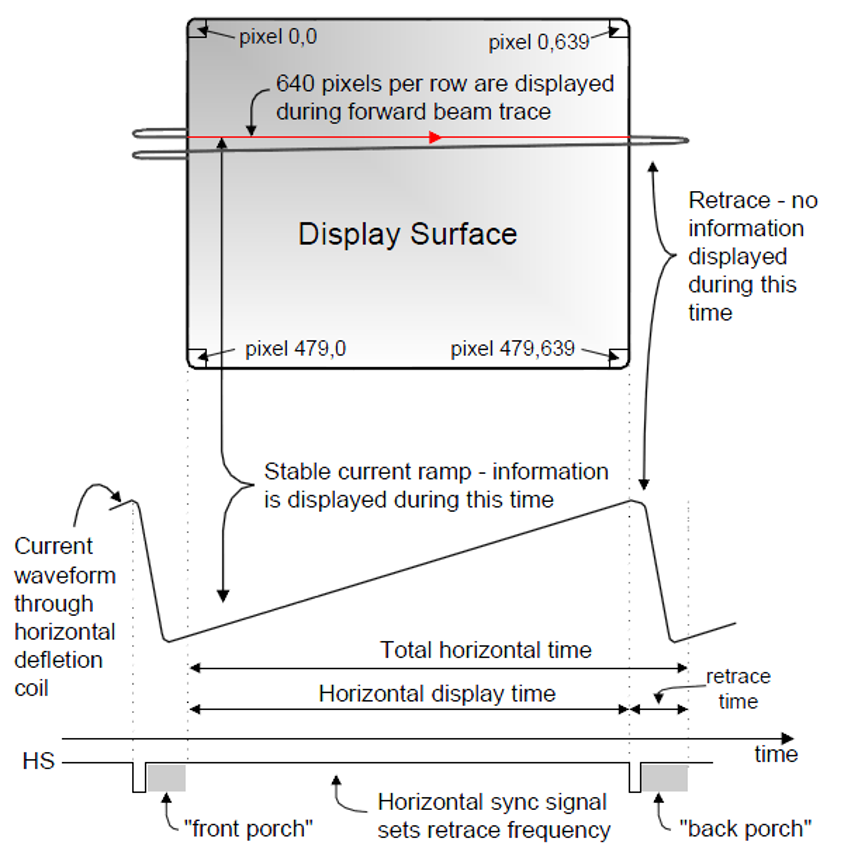
\includegraphics[width=1\linewidth]{report2-vga-scan1}
\caption{VGA 扫描}
\label{fig:report2-vga-scan1}
            \end{figure}

            对于640 × 480分辨率的图像,显示器的扫描过程如图\ref{fig:report2-vga-scan1}所示。
            
            VGA的时序包括水平时序和垂直时序,且两者都包含的时序参数有:水平(垂直)同步脉冲、水平(垂直)同步脉冲结束到有效显示数据区开始之间的宽度(后沿)、有效显示区宽度、有效数据显示区结束到水平(垂直)同步脉冲宽度开始之间的宽度(前沿)
            水平有效显示区宽度与垂直有效显示区宽度逻辑与的区域为可视区域,其他区域为消隐区。一行或一场的时序信息如图\ref{fig:report2-vga-scan2}所示。
            \begin{figure}
\centering

\includegraphics[width=1\linewidth]{report2-vga-scan2}
\caption{扫描信号}
\label{fig:report2-vga-scan2}
            \end{figure}
            
            VGA 的部分时许如表\ref{tab:vga-1}所示。
            \begin{sidewaystable}[h]
                \centering
                \begin{tabular}{|c|c|c|c|c|}
\hline 分辨率        & $640 \times  480$ & $800 \times  600$ & $1024 \times 768$ & $1280\times 1024$ \\
\hline 帧频(Hz)      & $60$ & $60$ & $60$ & $60$ \\
\hline 像素时钟(MHz) & $ 25.175$ & $ 40.0  $ & $ 65.0  $ & $108.0  $ \\
\hline 有效像素      &  640(pixel),  480(line) &  800(pixel),  600(line) & 1024(pixel),  768(line) & 1280(pixel), 1024(line) \\
\hline 前沿          & 16(pixel),11(line) & 40(pixel),1(line) & 24(pixel),3(line) & 48(pixel),1(line) \\
\hline 同步脉冲      & 96(pixel),2(line) & 128(pixel),4(line) & 136(pixel),6(line) & 112(pixel),3(line) \\
\hline 后沿          & 48(pixel),31(line) & 88(pixel),23(line) & 160(pixel),29(line) & 248(pixel),38(line) \\
\hline 总像素        & 800(pixel),524(line) & 1056(pixel),628(line) & 1344(pixel),806(line) & 1688(pixel),1066(line) \\
\hline
                \end{tabular} 
                \caption{部分VGA时序表}
                \label{tab:vga-1}
            \end{sidewaystable}
            
            
            模块划分如图\ref{fig:report2-vga-scan3}所示。
            \begin{figure}
\centering
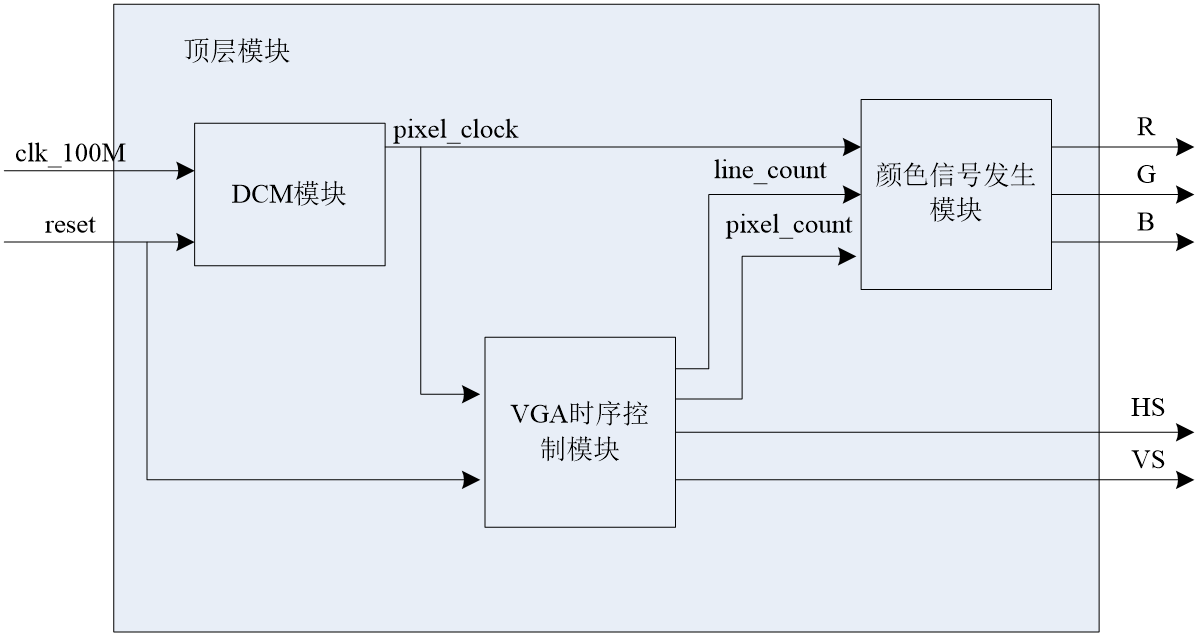
\includegraphics[width=1\linewidth]{report2-vga-scan3}
\caption{工程模块划分}
\label{fig:report2-vga-scan3}
            \end{figure}
            
            \subsubsection{实验步骤}
            \paragraph{新建工程}
            
            打开 ISE 14.7之后,选择新建工程,将工程的路径设置好。
            在单击下一步之后,选择 Nexys3 的 Spartan6 XC6SLX16-CS324 芯片对应的配置。硬件描述语言选择 Verilog,其中的设计硬件用的描述语言是 Verilog。
            然后点击下一步之后进入工程信息页面并确认无误之后,点击完成结束工程的创建。
            
            \paragraph{设计输入}
            
            在菜单 \verb|Project| 中选择 \verb|New Source| 创建新的设计,并选择 \verb|Verilog Module| 创建文件。
            
            其中输入的设计文件是:
            \begin{lstlisting}[language=Verilog,caption=SVGA\_DEFINES.v]
// Copyright (C) Xilinx
`define ZBT_PIPELINE_DELAY 	0		// not required for XUP-V2Pro
`define ZBT_INTERFACE_DELAY  	0	// not required for XUP-V2Pro
`define CHARACTER_DECODE_DELAY  4	// not required for XUP-V2Pro

/*
//  720 X 480 @ 50Hz with a 27MHz pixel clock for pal video capture
`define H_ACTIVE		720	// pixels
`define H_FRONT_PORCH	22	// pixels
`define H_SYNCH			64	// pixels
`define H_BACK_PORCH	58	// pixels
`define H_TOTAL		    864	// pixels

`define V_ACTIVE		576	// lines
`define V_FRONT_PORCH	6	// lines
`define V_SYNCH			6	// lines
`define V_BACK_PORCH	37	// lines
`define V_TOTAL			625	// lines
*/

/*
//  720 X 480 @ 60Hz with a 27MHz pixel clock for NTSC video capture
`define H_ACTIVE		720	// pixels
`define H_FRONT_PORCH	7	// pixels
`define H_SYNCH			62	// pixels
`define H_BACK_PORCH	69	// pixels
`define H_TOTAL		    858	// pixels

`define V_ACTIVE		487	// lines
`define V_FRONT_PORCH	4	// lines
`define V_SYNCH			4	// lines
`define V_BACK_PORCH	30	// lines
`define V_TOTAL			525	// lines
*/

/*
//  640 X 480 @ 60Hz with a 25.175MHz pixel clock
`define H_ACTIVE		640	// pixels
`define H_FRONT_PORCH	16	// pixels
`define H_SYNCH			96	// pixels
`define H_BACK_PORCH	48	// pixels
`define H_TOTAL			800	// pixels

`define V_ACTIVE		480	// lines
`define V_FRONT_PORCH	11	// lines
`define V_SYNCH			2	// lines
`define V_BACK_PORCH	31	// lines
`define V_TOTAL			524	// lines
*/

/*
//  640 X 480 @ 72Hz with a 31.500MHz pixel clock
`define H_ACTIVE		640	// pixels
`define H_FRONT_PORCH	24	// pixels
`define H_SYNCH			40	// pixels
`define H_BACK_PORCH	128	// pixels
`define H_TOTAL			832	// pixels

`define V_ACTIVE		480	// lines
`define V_FRONT_PORCH	9	// lines
`define V_SYNCH			3	// lines
`define V_BACK_PORCH	28	// lines
`define V_TOTAL			520	// lines
*/

/*
//  640 X 480 @ 75Hz with a 31.500MHz pixel clock
`define H_ACTIVE		640	// pixels
`define H_FRONT_PORCH	16	// pixels
`define H_SYNCH			96	// pixels
`define H_BACK_PORCH	48	// pixels
`define H_TOTAL			800	// pixels

`define V_ACTIVE		480	// lines
`define V_FRONT_PORCH	11	// lines
`define V_SYNCH			2	// lines
`define V_BACK_PORCH	32	// lines
`define V_TOTAL			525	// lines
*/

/*
// 640 X 480 @ 85Hz with a 36.000MHz pixel clock
`define H_ACTIVE		640	// pixels
`define H_FRONT_PORCH	32	// pixels
`define H_SYNCH			48	// pixels
`define H_BACK_PORCH	112	// pixels
`define H_TOTAL			832	// pixels

`define V_ACTIVE		480	// lines
`define V_FRONT_PORCH	1	// lines
`define V_SYNCH			3	// lines
`define V_BACK_PORCH	25	// lines
`define V_TOTAL			509	// lines
*/

/*
// 800 X 600 @ 56Hz with a 38.100MHz pixel clock
`define H_ACTIVE		800	// pixels
`define H_FRONT_PORCH	32	// pixels
`define H_SYNCH			128	// pixels
`define H_BACK_PORCH	128	// pixels
`define H_TOTAL			1088// pixels

`define V_ACTIVE		600	// lines
`define V_FRONT_PORCH	1	// lines
`define V_SYNCH			4	// lines
`define V_BACK_PORCH	14	// lines
`define V_TOTAL			619	// lines
*/

/*
// 800 X 600 @ 60Hz with a 40.000MHz pixel clock
`define H_ACTIVE		800	// pixels
`define H_FRONT_PORCH	40	// pixels
`define H_SYNCH			128	// pixels
`define H_BACK_PORCH	88	// pixels
`define H_TOTAL			1056// pixels

`define V_ACTIVE		600	// lines
`define V_FRONT_PORCH	1	// lines
`define V_SYNCH			4	// lines
`define V_BACK_PORCH	23	// lines
`define V_TOTAL			628	// lines
*/

/*
// 800 X 600 @ 72Hz with a 50.000MHz pixel clock
`define H_ACTIVE		800	// pixels
`define H_FRONT_PORCH	56	// pixels
`define H_SYNCH			120	// pixels
`define H_BACK_PORCH	64	// pixels
`define H_TOTAL			1040// pixels

`define V_ACTIVE		600	// lines
`define V_FRONT_PORCH	37	// lines
`define V_SYNCH			6	// lines
`define V_BACK_PORCH	23	// lines
`define V_TOTAL			666	// lines
*/

/*
// 800 X 600 @ 75Hz with a 49.500MHz pixel clock
`define H_ACTIVE		800	// pixels
`define H_FRONT_PORCH	16	// pixels
`define H_SYNCH			80	// pixels
`define H_BACK_PORCH	160	// pixels
`define H_TOTAL			1056// pixels

`define V_ACTIVE		600	// lines
`define V_FRONT_PORCH	1	// lines
`define V_SYNCH			2	// lines
`define V_BACK_PORCH	21	// lines
`define V_TOTAL			624	// lines
*/

/*
// 800 X 600 @ 85Hz with a 56.250MHz pixel clock
`define H_ACTIVE		800	// pixels
`define H_FRONT_PORCH	32	// pixels
`define H_SYNCH			64	// pixels
`define H_BACK_PORCH	152	// pixels
`define H_TOTAL			1048// pixels

`define V_ACTIVE		600	// lines
`define V_FRONT_PORCH	1	// lines
`define V_SYNCH			3	// lines
`define V_BACK_PORCH	27	// lines
`define V_TOTAL			631	// lines
*/


// 1024 X 768 @ 60Hz with a 65.000MHz pixel clock
`define H_ACTIVE		1024// pixels
`define H_FRONT_PORCH	24	// pixels
`define H_SYNCH			136	// pixels
`define H_BACK_PORCH	160	// pixels
`define H_TOTAL			1344// pixels

`define V_ACTIVE		768	// lines
`define V_FRONT_PORCH	3	// lines
`define V_SYNCH			6	// lines
`define V_BACK_PORCH	29	// lines
`define V_TOTAL			806	// lines


/*
// 1024 X 768 @ 70Hz with a 75.000MHz pixel clock
`define H_ACTIVE		1024// pixels
`define H_FRONT_PORCH	24	// pixels
`define H_SYNCH			136	// pixels
`define H_BACK_PORCH	144	// pixels
`define H_TOTAL			1328// pixels

`define V_ACTIVE		768	// lines
`define V_FRONT_PORCH	3	// lines
`define V_SYNCH			6	// lines
`define V_BACK_PORCH	29	// lines
`define V_TOTAL			806	// lines
*/

/*
// 1024 X 768 @ 75Hz with a 78.750MHz pixel clock
`define H_ACTIVE		1024// pixels
`define H_FRONT_PORCH	16	// pixels
`define H_SYNCH			96	// pixels
`define H_BACK_PORCH	176	// pixels
`define H_TOTAL			1312// pixels

`define V_ACTIVE		768	// lines
`define V_FRONT_PORCH	1	// lines
`define V_SYNCH			3	// lines
`define V_BACK_PORCH	28	// lines
`define V_TOTAL			800	// lines
*/

/*
// 1024 X 768 @ 85Hz with a 94.500MHz pixel clock
`define H_ACTIVE		1024// pixels
`define H_FRONT_PORCH	48	// pixels
`define H_SYNCH			96	// pixels
`define H_BACK_PORCH	208	// pixels
`define H_TOTAL			1376// pixels

`define V_ACTIVE		768	// lines
`define V_FRONT_PORCH	1	// lines
`define V_SYNCH			3	// lines
`define V_BACK_PORCH	36	// lines
`define V_TOTAL			808	// lines

*/
            \end{lstlisting}
            \begin{lstlisting}[language=Verilog,caption=vga\_timing.v]
`timescale 1ns / 1ps
// Copyright (C) Xilinx
`include "SVGA_DEFINES.v"

module vga_timing(
input clk,
input reset,
output reg hs,
output reg vs,
output reg [10:0] pixel_count,
output reg [9:0] line_count
);


//pixel counter
always @ (posedge clk or posedge reset) begin
if(reset) begin
pixel_count <= 0;
end
else begin
if(pixel_count == `H_TOTAL - 1) begin
pixel_count <= 0;
end
else begin
pixel_count <= pixel_count + 1;
end
end
end

// line counter
always @ (posedge clk or posedge reset) begin
if(reset) begin
line_count <= 0;
end
else begin
if(line_count == `V_TOTAL - 1 && pixel_count == `H_TOTAL - 1) begin
line_count <= 0;
end
else if(pixel_count == `H_TOTAL - 1) begin
line_count <= line_count + 1;
end
else begin
line_count <= line_count;
end
end
end

//产生行水平步信号
always @ (posedge clk or posedge reset) begin
if (reset) begin
hs <= 1'b1;
end

else if (pixel_count == (`H_ACTIVE + `H_FRONT_PORCH -1)) begin			
hs <= 1'b0;    // start of h_synch
end

else if (pixel_count == (`H_TOTAL - `H_BACK_PORCH -1)) begin
hs <= 1'b1;	  // end of h_synch
end

end

//产生垂直同步信号
always @ (posedge clk or posedge reset) begin
if (reset) begin
vs = 1'b1;			// remove v_synch
end

else if ((line_count == (`V_ACTIVE + `V_FRONT_PORCH -1) && (pixel_count == `H_TOTAL - 1))) begin
vs = 1'b0;		// start of v_synch
end

else if ((line_count == (`V_TOTAL - `V_BACK_PORCH - 1)) && (pixel_count == (`H_TOTAL - 1))) begin		
vs = 1'b1;	// end of v_synch
end
end
endmodule
            \end{lstlisting}
            \begin{lstlisting}[language=Verilog,caption=color\_gen.v]
`timescale 1ns / 1ps
//Copyright (C) Xilinx
`include "SVGA_DEFINES.v"

module color_gen(
clk,
reset,
format_sel,
pixel_count,
line_count,
RED,
GREEN,
BLUE
);

input clk;
input reset;
input format_sel;
input [10:0] pixel_count;
input [9:0] line_count;

output reg [2:0] RED;
output reg [2:0] GREEN;
output reg [1:0] BLUE;

reg color_valid;

always @ (pixel_count or line_count) begin
if(pixel_count >= 0 && pixel_count <= `H_ACTIVE - 1) begin
if(line_count >= 0 && line_count <= `V_ACTIVE - 1) begin
color_valid = 1'b1;
end
else begin
color_valid = 1'b0;
end
end
else begin
color_valid = 1'b0;
end
end

//产生彩条图形
always @ (posedge clk or posedge reset) begin
if(reset) begin
RED <= 3'b111;
GREEN <= 3'b111;
BLUE <= 2'b11;
end
else begin
if(format_sel == 1'b1) begin	//横彩条
if(color_valid == 1'b1) begin
if(line_count >= 0 && line_count < `V_ACTIVE/4) begin
//红
RED <= 3'b111;
GREEN <= 3'b00;
BLUE <= 2'b00;
end
else if(line_count >= `V_ACTIVE/4 && line_count < `V_ACTIVE/2)begin
//绿
RED <= 3'b000;
GREEN <= 3'b111;
BLUE <= 2'b00;
end
else if(line_count >= `V_ACTIVE/2 && line_count < `V_ACTIVE/4*3) begin
//蓝
RED <= 3'b000;
GREEN <= 3'b000;
BLUE <= 2'b11;
end
else begin
//白
RED <= 3'b111;
GREEN <= 3'b111;
BLUE <= 2'b111;
end
end
else begin
RED <= 3'b000;
GREEN <= 3'b000;
BLUE <= 2'b00;
end
end
else begin	//竖彩条
if(color_valid) begin
if(pixel_count >= 0 && pixel_count < `H_ACTIVE/4) begin
//品红
RED <= 3'b111;
GREEN <= 3'b000;
BLUE <= 2'b11;
end
else if(pixel_count >= `H_ACTIVE/4 && pixel_count < `H_ACTIVE/2) begin
//黄
RED <= 3'b111;
GREEN <= 3'b111;
BLUE <= 2'b00;
end
else if(pixel_count >= `H_ACTIVE/2 && pixel_count < `H_ACTIVE*3/4) begin
//青
RED <= 3'b000;
GREEN <= 3'b111;
BLUE <= 2'b11;
end
else begin
//黑
RED <= 3'b000;
GREEN <= 3'b000;
BLUE <= 2'b00;
end
end
else begin
RED <= 3'b000;
GREEN <= 3'b000;
BLUE <= 2'b00;
end
end
end
end
endmodule
            \end{lstlisting}
            \begin{lstlisting}[language=Verilog,caption=VGA\_display.v]
`timescale 1ns / 1ps
// Copyright (C) Xilinx
`include "SVGA_DEFINES.v"

module VGA_display(
clk_100M,
reset,
format_sel,
RED,
GREEN,
BLUE,
HSYNC,
VSYNC
);

input clk_100M;
input reset;
input format_sel;
output [2:0] RED;
output [2:0] GREEN;
output [1:0] BLUE;
output HSYNC;
output VSYNC;

wire pixel_clock;
wire locked;

wire [10:0] pixel_count;
wire [9:0] line_count;

wire hs;
wire vs;

dcm_dsgn dcm0
(// Clock in ports
.CLK_IN1(clk_100M),      // IN
// Clock out ports
.CLK_OUT1(pixel_clock),     // OUT
// Status and control signals
.RESET(reset),// IN
.LOCKED(locked));      // OUT


vga_timing vga_timing_gen (
.clk(pixel_clock), 
.reset(reset), 
.hs(hs), 
.vs(vs), 
.pixel_count(pixel_count), 
.line_count(line_count)
);


assign HSYNC = hs;
assign VSYNC = vs;

// Instantiate the module
color_gen color_gen0 (
.clk(pixel_clock), 
.reset(reset), 
.format_sel(format_sel), 
.pixel_count(pixel_count), 
.line_count(line_count), 
.RED(RED), 
.GREEN(GREEN), 
.BLUE(BLUE)
);
endmodule
            \end{lstlisting}
            
            然后在创建一个时钟IP核的实例,并将输出频率设置为65MHz。
            然后添加约束文件,如下
            \begin{lstlisting}[caption=约束文件]
## VGA Connector
NET RED[0] LOC = U7 | IOSTANDARD = LVCMOS33; # Bank = 2, pin name = IO_L43P, Sch name = RED0
NET RED[1] LOC = V7 | IOSTANDARD = LVCMOS33; # Bank = 2, pin name = IO_L43N, Sch name = RED1
NET RED[2] LOC = N7 | IOSTANDARD = LVCMOS33; # Bank = 2, pin name = IO_L44P, Sch name = RED2
NET GREEN[0] LOC = P8 | IOSTANDARD = LVCMOS33; # Bank = 2, pin name = IO_L44N, Sch name = GRN0
NET GREEN[1] LOC = T6 | IOSTANDARD = LVCMOS33; # Bank = 2, pin name = IO_L45P, Sch name = GRN1
NET GREEN[2] LOC = V6 | IOSTANDARD = LVCMOS33; # Bank = 2, pin name = IO_L45N, Sch name = GRN2
NET BLUE[0] LOC = R7 | IOSTANDARD = LVCMOS33; # Bank = 2, pin name = IO_L46P, Sch name = BLU1
NET BLUE[1] LOC = T7 | IOSTANDARD = LVCMOS33; # Bank = 2, pin name = IO_L46N, Sch name = BLU2

NET "HSYNC" LOC = N6 | IOSTANDARD = LVCMOS33; # Bank = 2, pin name = IO_L47P, Sch name = HSYNC
NET "VSYNC" LOC = P7 | IOSTANDARD = LVCMOS33; # Bank = 2, pin name = IO_L47N, Sch name = VSYNC

NET "clk_100M" LOC= V10 | IOSTANDARD = LVCMOS33;
NET "reset" LOC = C9 | IOSTANDARD = LVCMOS33;
NET "format_sel" LOC = T10 | IOSTANDARD = LVCMOS33;
            \end{lstlisting}
            
            \paragraph{综合实现}
            分别依次双击\verb|Synthesize-XST| 与 \verb|Implement Design| 进行综合实现。
            
            \paragraph{器件配置}
            双击 \verb|Generate Programming File| 生成比特流文件,启动开发板并将与显示器链接。
            然后双击\verb|Configure Target Device| 配置设备。
            
            \subsubsection{结果}
            显示器最后输出的结果如图\ref{fig:report2-vga-scan4} 与 图\ref{fig:report2-vga-scan5}        
            \begin{figure}[h]
\centering
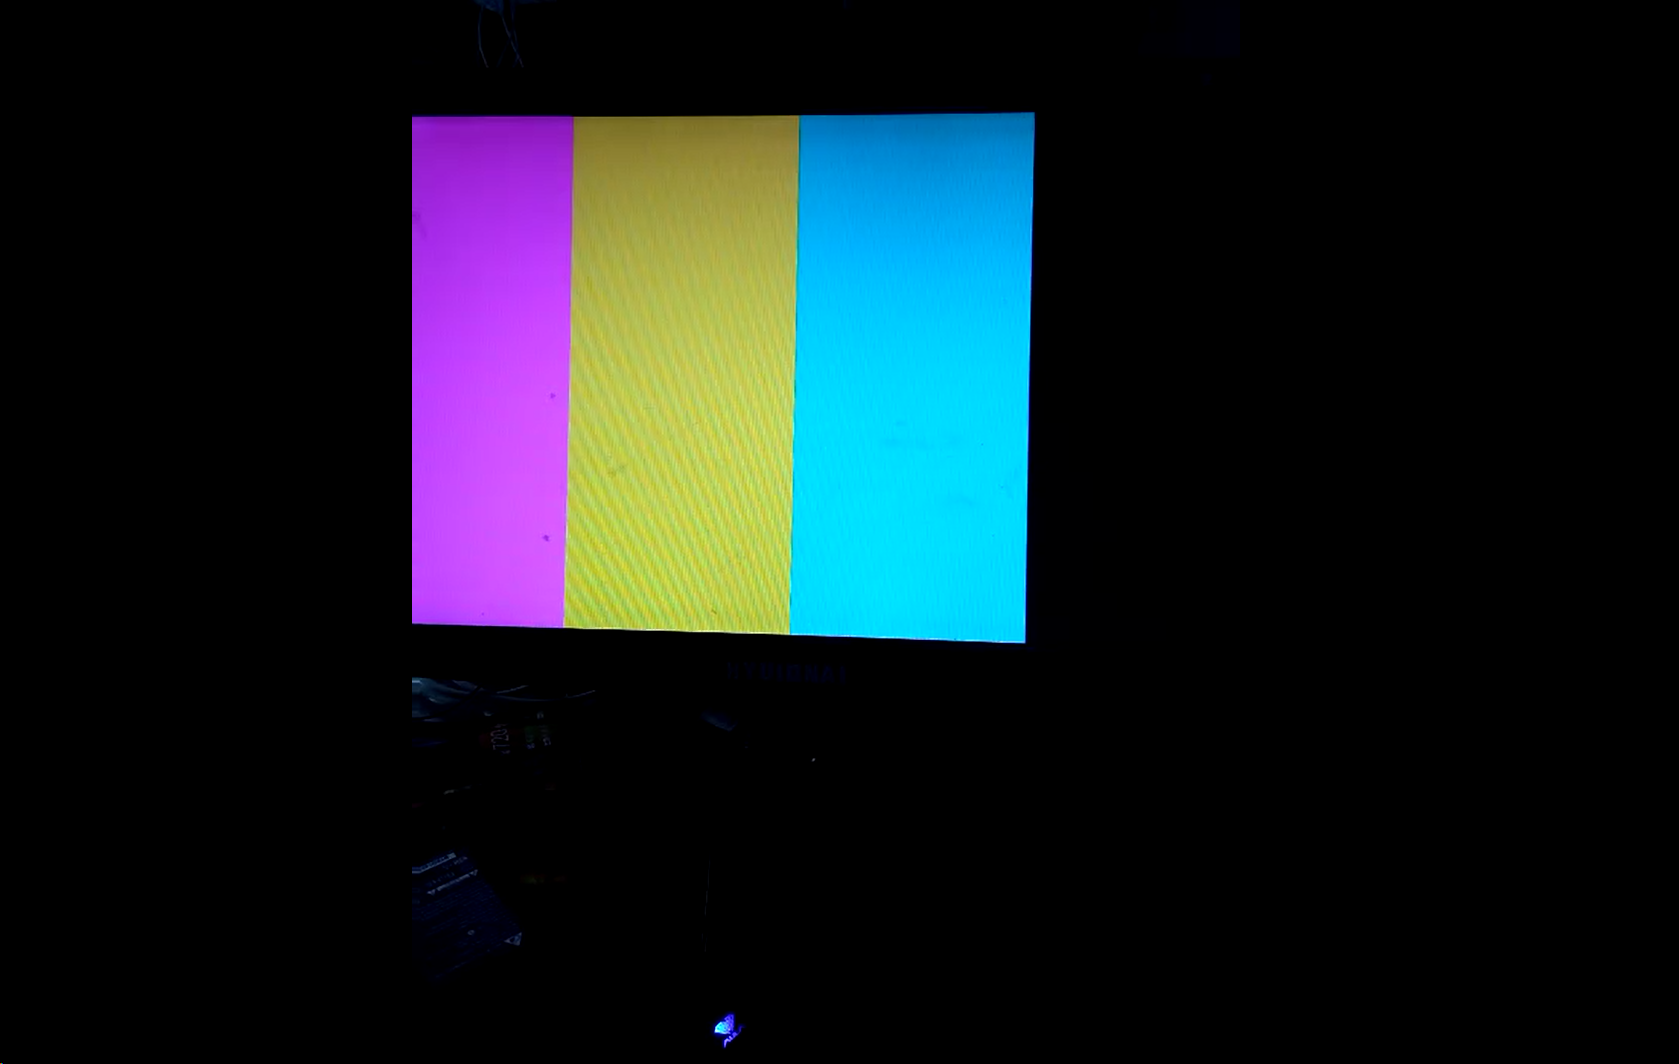
\includegraphics[width=1\linewidth]{report2-vga-scan4}
\caption{输出}
\label{fig:report2-vga-scan4}
\end{figure}
\begin{figure}[h]
\centering
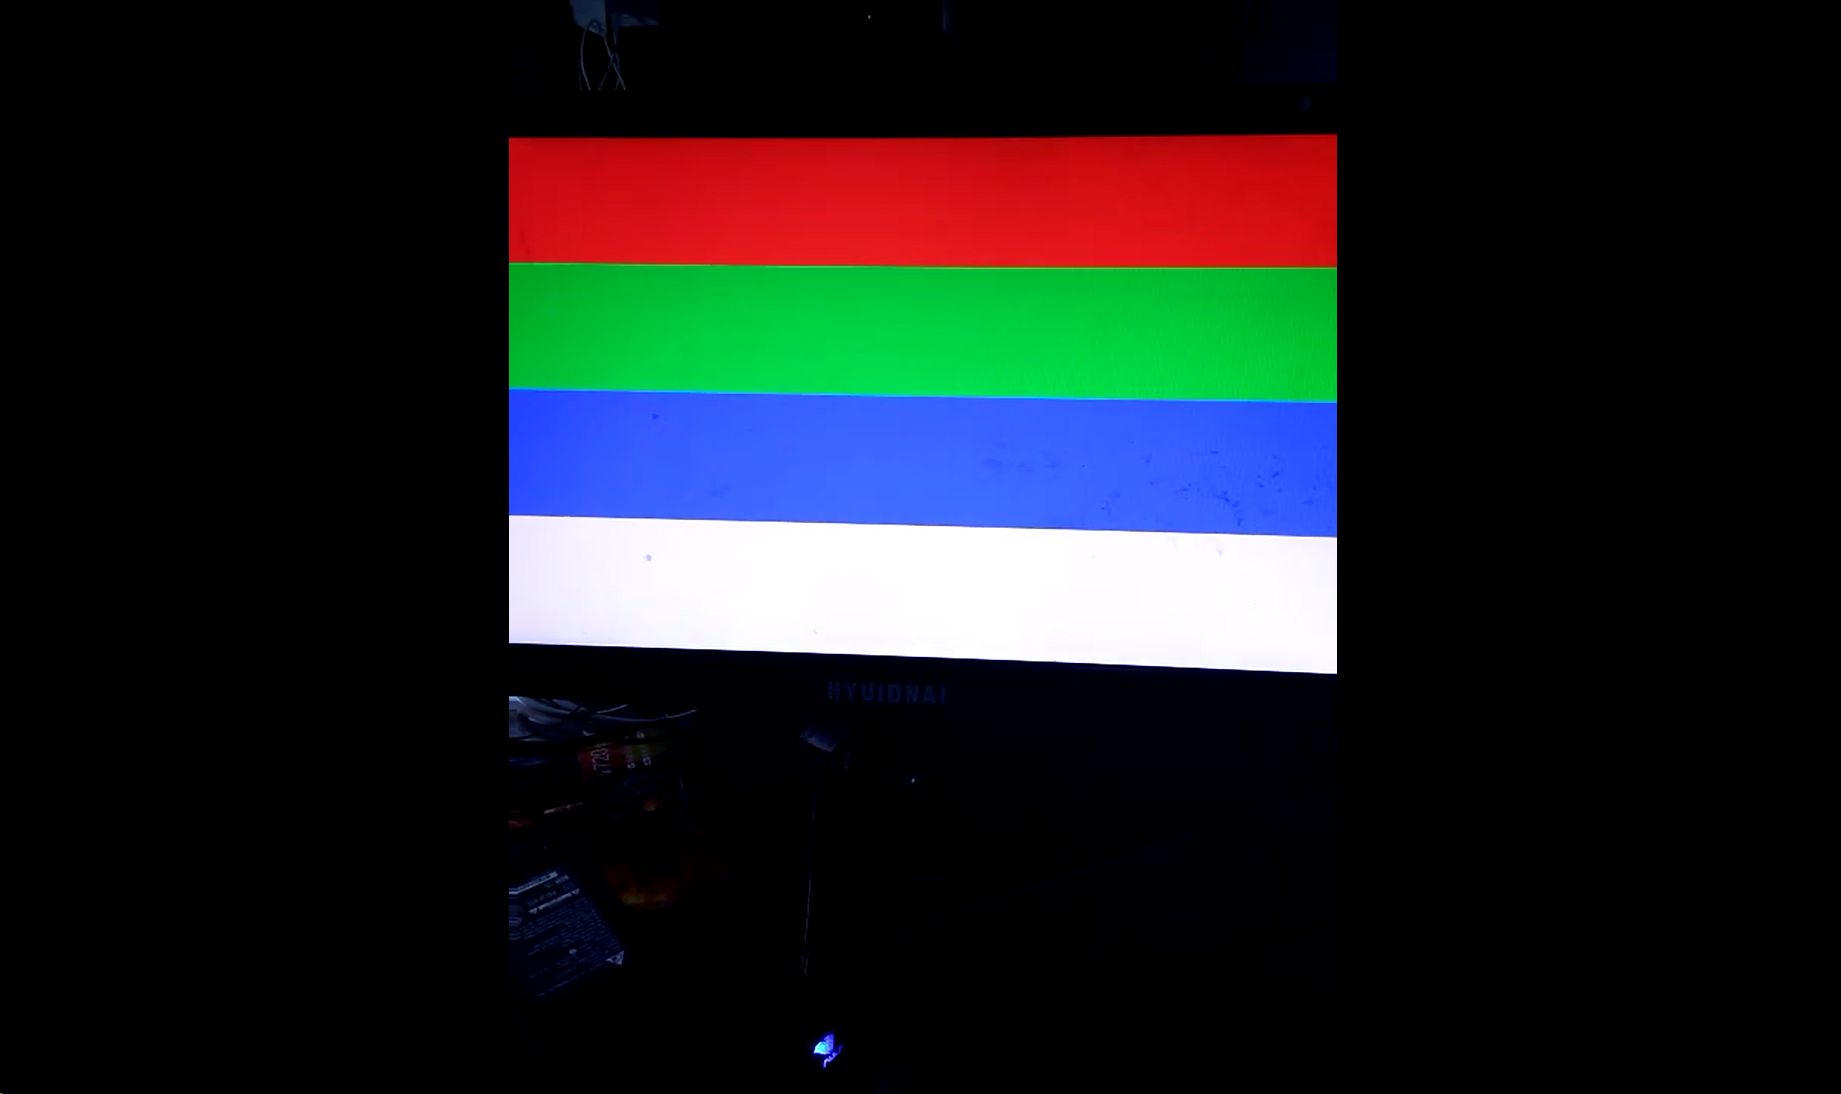
\includegraphics[width=1\linewidth]{report2-vga-scan5}
\caption{输出}
\label{fig:report2-vga-scan5}
\end{figure}

\end{document}